\chapter{評価実験}
\label{chap:main_experiment}

この章では本研究で行った評価実験について述べる.

\section{評価実験の概要}
\section{評価実験の目的}
\section{ORF(Open Research Forum)におけるデータ収集}
\section{ユーザーの嗜好分析}

\begin{figure}[htbp]
    \begin{center}
       \fbox{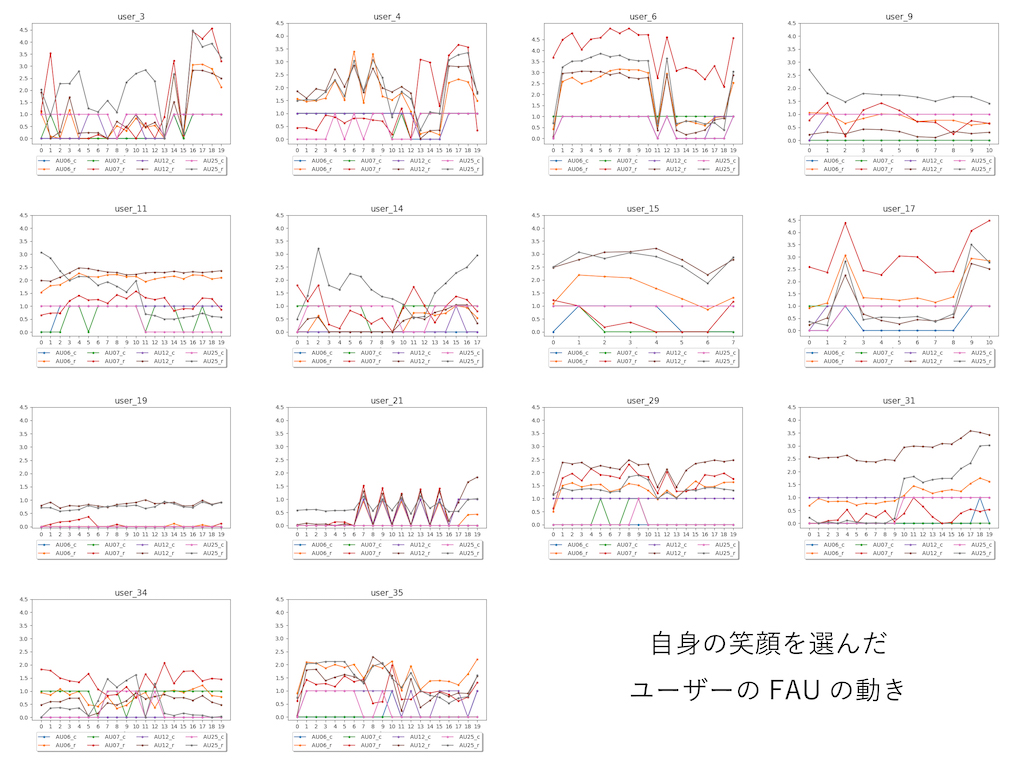
\includegraphics[width=150mm,bb=0 0 1024 768]{choice_myself_fau_for_paper.jpg}}
    \end{center}
    \caption{自身を選択したユーザーのFAUデータ}
    \label{fig:choice_myself_fau_for_paper}
\end{figure}

\begin{figure}[htbp]
    \begin{center}
       \fbox{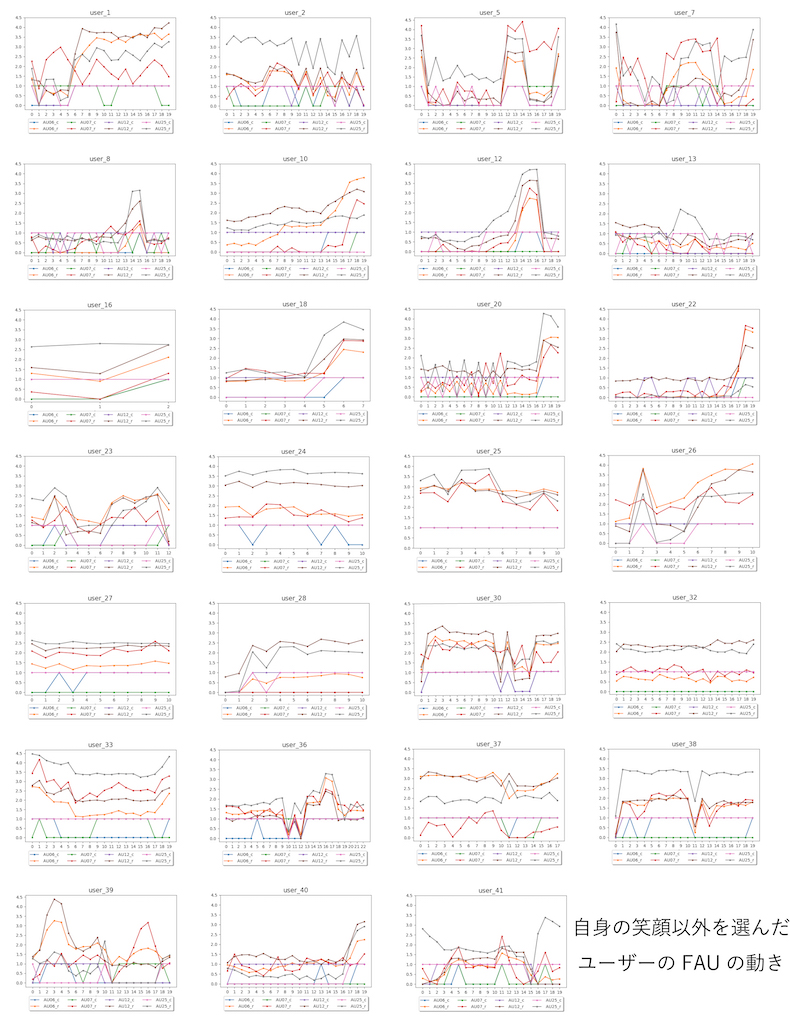
\includegraphics[width=150mm,bb=0 0 790 1024]{choose_else_for_paper.jpg}}
    \end{center}
    \caption{自身を選択しなかったユーザーのFAUデータ}
    \label{fig:choose_else_for_paper}
\end{figure}

\begin{figure}[htbp]
    \begin{center}
       \fbox{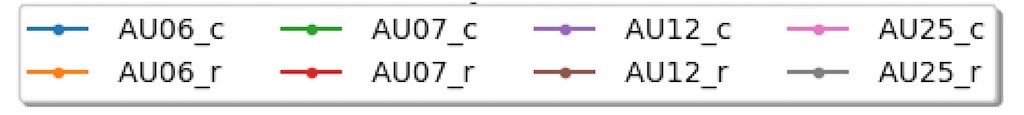
\includegraphics[width=150mm,bb=0 0 1024 115]{usage_guide_fau.jpg}}
    \end{center}
    \caption{ユーザーFAUグラフ凡例}
    \label{fig:usage_guide_fau}
\end{figure}

\section{自身の表情の作り方と好感をもつ笑顔との相関性}
\section{結果}
\section{まとめ}
